%!TEX root = paper.tex
%
% AMRClaw
%
% Lead currently:  Marsha Berger
%

\subsection{\amrclaw}\label{sec:amrclaw}
Fortran code in the \amrclaw repository performs block structured adaptive mesh
refinement \cite{BO,BC} for both 
\clawpack and \geoclaw  applications.
A short overview is given
here to set the stage for a description of recent changes.
\amrclaw includes the functionality for: 
\begin{itemize}
\item
coordinating the flagging of points where refinement is needed,
with a variety of criteria possible for flagging cells that need refinement
from each level to the next finer level (including Richardson extrapolation,
gradient testing, or user-specified criteria).  See
\url{http://www.clawpack.org/flag.html};
\item
organizing the flagged points into efficient grid
patches at the next finer level, using the algorithm of
\cite{mjb-rig:cluster};
\item
initializing newly created fine grids, both solution and auxiliary arrays that store additional grid data such as topography, wind velocity, metric data for example latitude and longitude, etc.;
\item
orchestrating the time stepping, since refinement levels may have
different time steps ({called sub-cycling in time});
\item
interpolating for ghost cells at the boundaries of fine patches,
needed before a time step can be taken;
\item
updating coarse grid values covered by finer grid patches;
\item
maintaining conservation at patch boundaries between resolution levels.
\end{itemize}
The algorithms implemented in \amrclaw have been discussed in detail in
\cite{mjb-rjl:amrclaw,LeVequeGeorgeBerger:an11}. 

\amrclaw now allows users to specify ``regions'' in space-time 
$[x_1,x_2] \times [y_1,y_2] \times [t_1,t_2]$ in which refinement is forced to
be at least at some level $L_1$ and is allowed to be at most $L_2$.  This can be
useful for constraining refinement, e.g. allowing or ensuring resolution of only a small coastal region in a global tsunami simulation.
Previously the user could enforce such conditions by writing a custom
flagging routine, but now this is handled in a general manner so that the
parameters above can all be specified in \texttt{setrun.py}.  Multiple
regions can be specified, and a simple rule is used to determine the
constraints at a grid cell that lies in multiple regions, as described at
\url{http://www.clawpack.org/flag.html#refinement-regions}

Auxiliary arrays are often used in \clawpack to store data that 
describes the problem and the routine.
The routine \texttt{setaux} must then be provided by the user to set these values each time a
new grid patch is created.  For some applications computing these values can be time-consuming.  In \clawpack 5.2,
this code was improved to allow reuse of values from previous patches at
the same level where possible at each regridding time. 
This is backward compatible, since no harm is done if previously
written routines are used that still compute and overwrite instead of
checking a mask.  

In \clawpack 5.3 the capability to specify spatially varying boundary conditions
was added. For a single grid, it is a simple matter to
compute the location of the ghost cells that extend
outside the computational domain and set them appropriately.
With AMR however, the boundary condition routine can be called
for a grid located anywhere in the domain, and may contain fewer
or larger numbers of ghost cells. The boundary condition routines
must be written in a rather unusual way that does not assume it
is always setting the same number of ghost cells, or that the
same number of reflected cells inside the domain always exist.

Anisotropic refinement is allowed in both two and three dimensions.  This means that the spatial and temporal refinement ratios can be specified independently from one another (as long as the temporal refinement satisfies the CFL condition).
In addition, capabilities have been added to automatically select the 
refinement ratio on each level based on the CFL condition.

The 3D \amrclaw code has been reintroduced in 5.0. \amrclaw has also been
parallelized using OpenMP directives based on grid patch-based decomposition.
The main paradigm in structured AMR is a loop over all patches at a level, where
some operation is done on each patch (i.e. taking a time step, finding ghost
cells, conservation updates, etc.).  This lends itself easily to a {\tt parallel
for} loop construct where each iteration of the loop corresponds to a grid at
that level. Dynamic scheduling is used with a chunk size of one, so that one
thread is assigned one patch at a time. To help with load balancing, patches at
each level are sorted from largest to smallest workload when they are first
created, using the total number of cells in the grid as an indicator of work.
Note that this approach causes a memory bulge. Each thread must have its own
scratch arrays to save the incoming and outgoing waves and fluxes for future
conservation fix-ups. The bulge is directly proportional to the number of
threads executing. For stack-based memory allocation per thread, the use of the
environment variable {\tt OMP\_STACKSIZE} to increase the limit may be
necessary.

The parallelization of \amrclaw and \geoclaw assumes multi-core machines for the
target architecture.  \pyclaw, on the other hand, does not include AMR but uses
MPI via PETSc to achieve parallelism on distributed memory machines that scale
to tens of thousands of cores (see \cref{sec:pyclaw}). Other frameworks exist,
most notably \forestclaw \cite{Burstedde:we} which are being developed in
parallel with \amrclaw to provide scalable AMR calculations on large distributed
memory machines. \todo{Need to cite \cref{fig:figure1} and add caption.}

\begin{figure}[h]
    \centering
    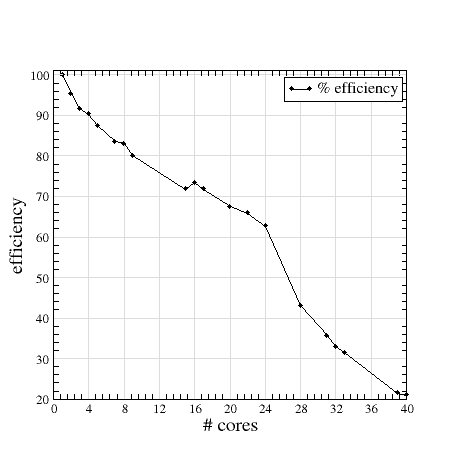
\includegraphics[width=0.45\textwidth]{efficiency}
    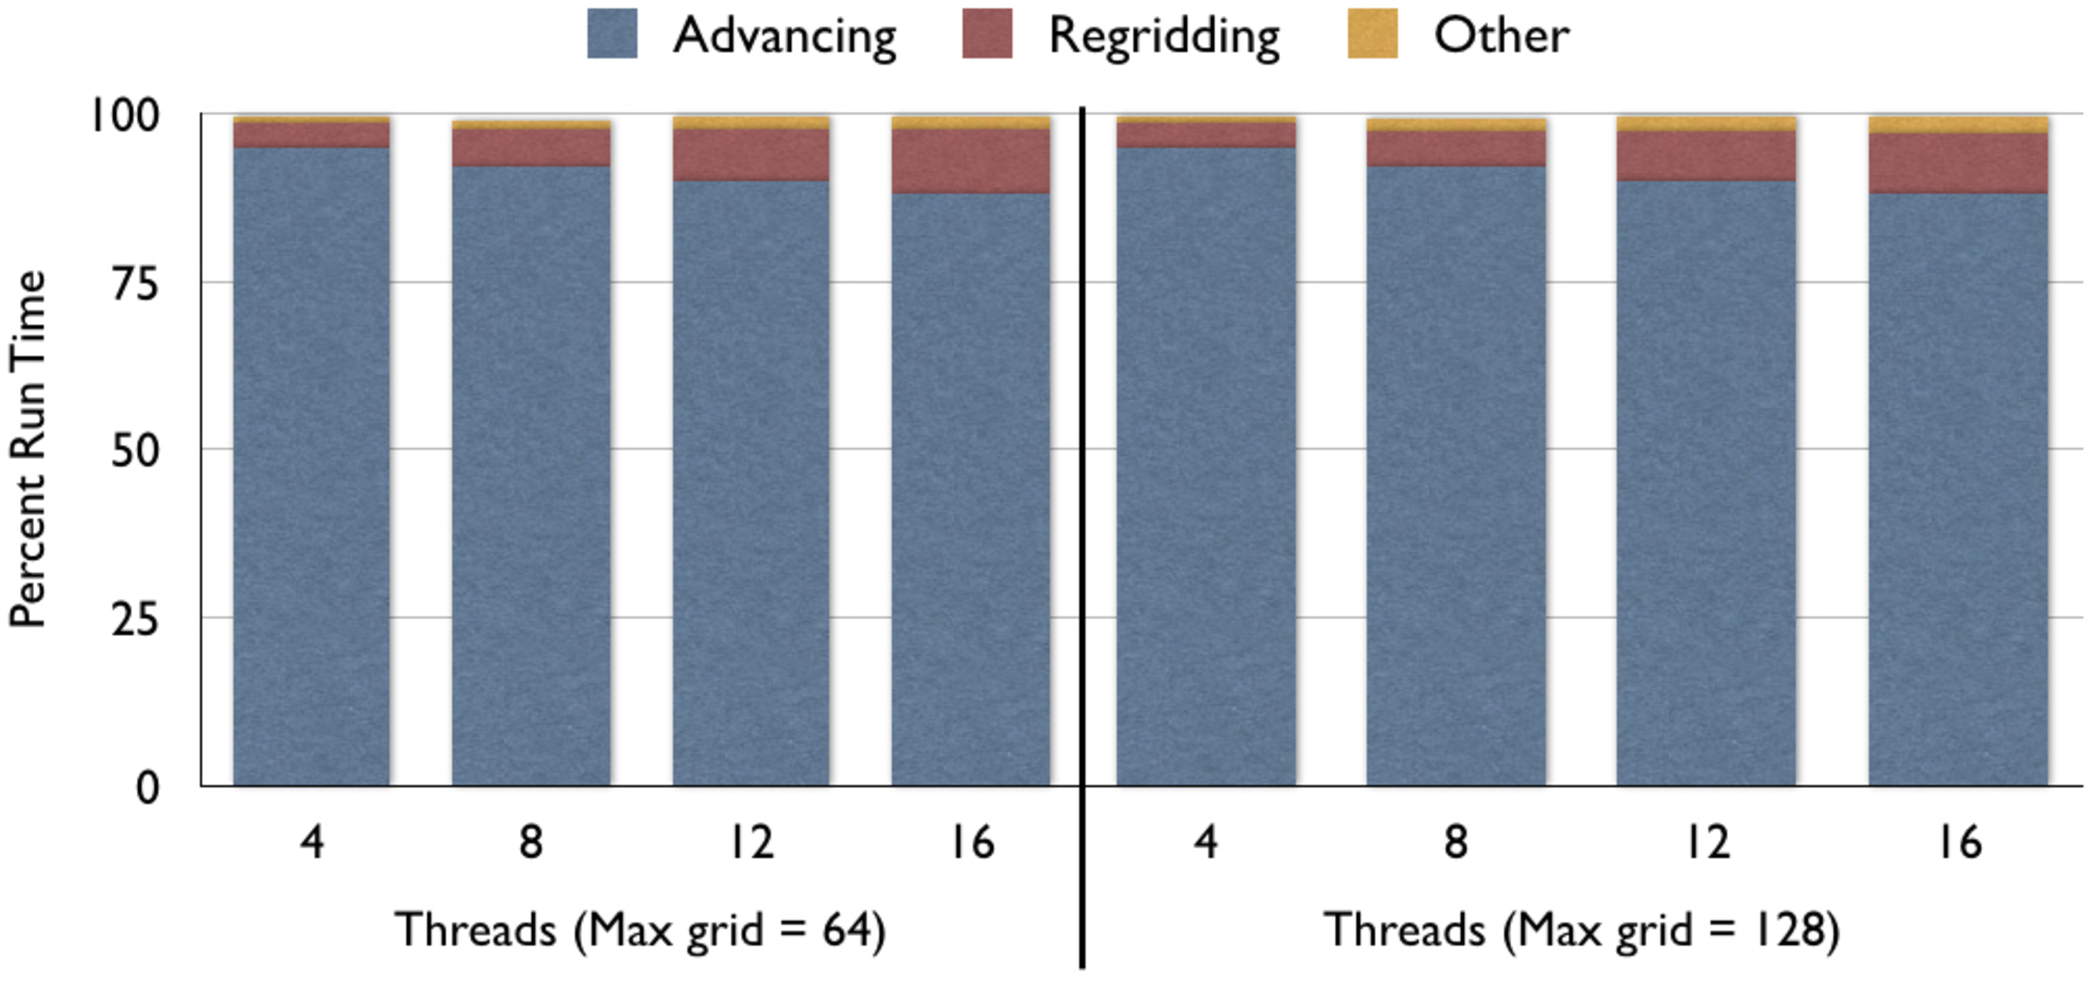
\includegraphics[width=0.45\textwidth]{weak_scaling}
    \caption{Caption here.}
    \label{fig:figure1}
\end{figure}
